%\documentclass{sig-alternate}
\documentclass{acm_proc_article-sp}

\begin{document}

\title{High Confidence Embedded Software Design: A Quadrotor Helicopter Case Study}

\numberofauthors{5}
\author{
% 1st. author
\alignauthor Zhenkai Zhang
%\email{zhenkai.zhang@vanderbilt.edu}
% 2nd. author
\alignauthor Joseph Porter
%\email{jporter@isis.vanderbilt.edu}
% 3rd. author
\alignauthor Nicholas Kottenstette
%\email{nkottens@isis.vanderbilt.edu}
\and  % use '\and' if you need 'another row' of author names
% 4th. author
\alignauthor Xenofon Koutsoukos
%\email{xenofon.koutsoukos@vanderbilt.edu}
% 5th. author
\alignauthor Janos Sztipanovits
%\email{janos.sztipanovits@vanderbilt.edu}
\and
\affaddr{Institute for Software Integrated Systems (ISIS)}\\
\affaddr{Department of Electrical Engineering and Computer Science}\\
\affaddr{Vanderbilt University}\\
\affaddr{Nashville, TN, USA}\\
\email{zhenkai.zhang@vanderbilt.edu}
}


\maketitle
\begin{abstract}
Traditional design methodology is not suitable for high-confidence embedded software due to the lack of a formal semantic model for software analysis, automatic code generation, and often designed embedded software is hard to reuse. In order to automatically generate high-confidence and reusable embedded software, we propose a TLM-centric, platform-based, time-triggered and component-oriented method. We use this new method to generate the control software for a quadrotor helicopter.
\end{abstract}

% A category with the (minimum) three required fields
\category{H.4}{Information Systems Applications}{Miscellaneous}
%A category including the fourth, optional field follows...
\category{D.2.8}{Software Engineering}{Metrics}[complexity measures, performance measures]

\terms{Theory}

\keywords{Computer aided software engineering, Real-time systems, Embedded software, Digital control, Graphical models, Metamodeling} % NOT required for Proceedings

\section{Introduction}
In many cyber-physical systems (CPS), how to automatically analyze and generate high-confidence embedded software becomes a key issue. High-confidence embedded software is needed in hard real-time systems, e.g. safety-critical systems. Moreover, designers also want to reuse successful software to save money and energy, and most importantly, to save time-to-market. However, there are some drawbacks that impede the automatic analysis, generation and reuse of embedded software: (1) Generating high-confidence embedded software requires a formal model (or models) containing the necessary semantics to enable software analysis; (2) Embedded software needs to be integrated with the underlying hardware, and the integration makes embedded software hard to develop, analyze, and reuse; (3) Timing requirements and software performance vary among different systems, so porting the software to another system might violate timing requirements; (4) When trying to port monolithic embedded software to a distributed system, it is hard to guarantee some correctness properties will remain (e.g. determinism and deadlock freedom).

In order to have a model containing all the semantics for automatic generation, deal with this tight coupling to the underlying hardware, make the timing of the embedded software easy to be analyzed and controlled, and provide a solution for distributed systems, many new design methods have been proposed. Among the model-based design methods, the \emph{Transaction-Level Modeling} (TLM) is systematic and suitable for automatic code generation \cite{modeling:embedded}\cite{modeling:tlm}. For dealing with tight coupling to the underlying hardware, platform-based design provides an abstraction layer that hides the details of several possible low-level refinements \cite{modeling:platform}. Time-triggered architecture is a particular platform abstraction which is used to analyze timing behavior of embedded software \cite{modeling:giotto3}. Actor-oriented design provides a method that specifies formal models of computation for execution of distributed components \cite{embedded:software}.

Although many different issues can be addressed by using these different methods, there is little work considering all these design concerns for a specific application. In order to automatically generate high-confidence and reusable embedded software, we propose a TLM-centric, platform-based, time-triggered and component-oriented method, and we use this new method to generate the control software for a quadrotor helicopter.


\section{Overview}
In our method, we start with a specification model (SM) of the control system using Simulink. After validation of this SM by simulation, we import the model into an automated embedded software development environment. The environment uses a suite of domain-specific modeling languages (DSMLs) called the Embedded Systems Modeling Language (ESMoL) to integrate analysis and code generation tools. In the ESMoL environment, we establish a TLM based on the imported SM. The TLM captures the hardware platform of the system, the mapping of tasks to the processors and messages to the communication ports, and the scheduling information of the tasks. Based on this TLM, we perform embedded software synthesis which consists of code generation and binary generation. We evaluate the binary code on the target platform to check performance with requirements.

ESMoL is a suite of DSMLs which function together as a system level design language (SLDL), providing a single multi-aspect design environment. Modeling, analysis, simulation, and code generation are all related to a single design model. The design language is specific to distributed embedded control systems, and is described in \cite{modeling:esmol}.

\begin{figure}[!t]
\centering
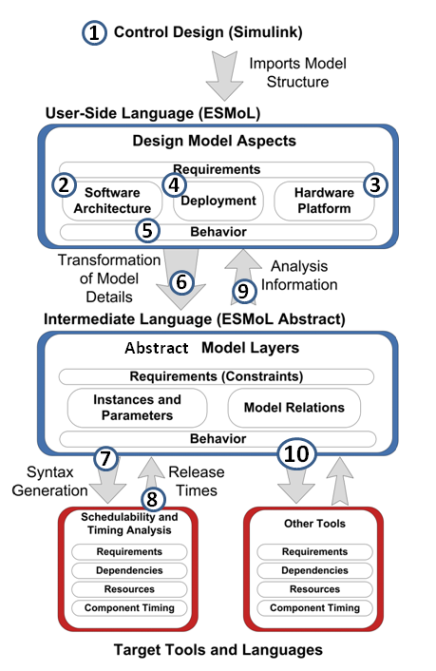
\includegraphics[width=0.80\columnwidth]{figures/designflow.png}
\caption{Design flow supported by the ESMoL language and modeling tools.}
\label{fig:designflow}
\end{figure}

According to \cite{modeling:esmol}, we follow the design flow shown in Fig. \ref{fig:designflow}. Step 1 is to specify the control system's functionality in the Simulink environment. After validation of this control system design, the model can be imported automatically into the ESMoL environment. The Simulink model will become a synchronous dataflow model (SDF), and each subsystem in the Simulink model becomes an actor in the SDF \cite{moc:sdf}. ESMoL model references to imported Simulink blocks become the functional specifications for instances of software components in a logical SDF model. C code fragments may also be used to specify component functionality. Component ports (shown in Fig. \ref{fig:QuadrotorLogicalSoftwareArchitecture}) represent instances of data message types. These types are defined as structures with individual data fields to which Simulink data ports can be mapped. These relations describe the marshaling, demarshaling, and transfer of data between software components \cite{modeling:esmol}.

Step 2 is to specify the logical software architecture which captures data dependencies between software component instances independent of their distribution over different processors.

Step 3 is to define hardware platforms hierarchically as hardware units with ports for interconnections. Primitive components include processing nodes and communication buses. Behavioral semantics for these network models come from the underlying time-triggered architecture. The time-triggered platform provides services such as deterministic execution of replicated components and timed message-passing. Model attributes for hardware also capture timing resolution, overhead parameters for data transfers, and task context switching times \cite{modeling:esmol}.

Step 4 is to set up a deployment model by mapping software components to processing nodes, and data messages to communication ports. The deployment model captures the assignment of component instances as periodic tasks running on a particular processor. In ESMoL a task executes on a processing node at a single periodic rate. All components within the task execute synchronously. Message ports on component instances are assigned to hardware interface ports in the model to define the media through which messages are transferred \cite{modeling:esmol}.

Step 5 is to establish a timing model by attaching timing parameter blocks to components and messages. For the time-triggered case the configuration parameters include execution period and worst-case execution time. The execution model also indicates which components and messages will be scheduled independently, and which will be grouped into a single task or message object \cite{modeling:esmol}.

The TLM scheduling information is added in step 6 through step 9. Step 6 translates an ESMoL model into the simpler ESMoL\_Abstract model using the Stage 1 model transformation described in \cite{modeling:esmol}. Step 7 is to use the equivalent model in ESMoL\_Abstract to generate a scheduling problem specification according to a template. In step 8 a tool called \emph{SchedTool} solves the generated scheduling problem. Step 9 is to import the results back into the ESMoL model and write them to the appropriate objects. For more details, please refer to \cite{modeling:esmol}. Step 10 is to generate the corresponding C code, which will be described in next section.


\section{Modeling and Code Generation}

We use the above approach to design and implement the embedded software for a quadrotor helicopter. Quadrotor helicopters are agile aircraft which are lifted and propelled by four rotors. Because their attitude dynamics change so quickly, it is difficult if not impossible for a human to successfully fly and maneuver such vehicles \cite{quad:passcontrol}. Thus, these aircraft need an automated control system to help them fly. The controller, software and hardware design domains are highly specialized and conceptually incompatible. For example, control theory deals with a continuous system, software design is for a discrete environment, and computing hardware must deal with both. This makes effectively and efficiently implementing such a high confidence embedded control system significantly difficult.

\subsection{Simulink model of the quadrotor's control system}

The control design for the quadrotor helicopter is introduced in \cite{quad:passcontrol}, which uses passive attitude control. Specifically, two linear proportional derivative (PD) controllers are used, an inner loop and an outer loop. The outer loop controller is a ``fast'' PD inertial controller and the inner loop is a ``fast'' PD attitude controller.

The on-board sensors include a GPS and an IMU. In the Simulink model we do not capture the behavior and interfaces of the particular sensor chips, so their receiving message types are modeled not specifically but universally. The controller takes x, y, and z coordinates instead of longitude, latitude and height as position, so a specific subsystem \emph{Sensor\_Convert} is added to make the conversion. The \emph{Outer\_Loop} subsystem is for inertial position control and \emph{Inner\_Loop} is for attitude control. \emph{Reference\_Handler} is used to receive and handle destinations, and \emph{Plant\_Dynamics} is used to simulate the behavior (not realized as a software component).

\subsection{Logical software architecture of the control system}

\begin{figure}[!t]
\centering
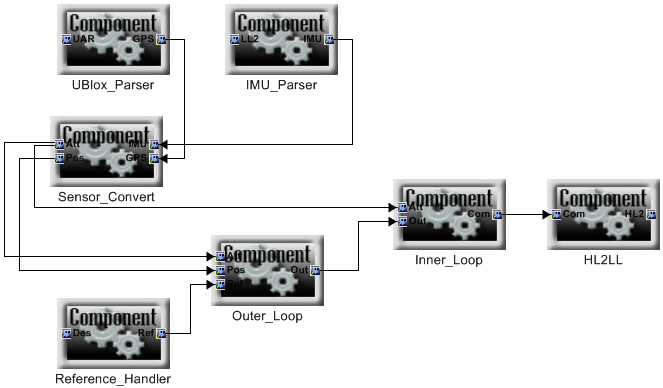
\includegraphics[width=\columnwidth]{figures/QuadrotorLogicalSoftwareArchitecture.png}
\caption{The logical software architecture for quadrotor's control system.}
\label{fig:QuadrotorLogicalSoftwareArchitecture}
\end{figure}

Fig. \ref{fig:QuadrotorLogicalSoftwareArchitecture} shows logical data dependencies between software component instances. To establish functional determinism and deadlock freedom, we analyze the imported Simulink blocks in the logical architecture model as a SDF model. SDF guarantees that each actor (corresponding to a subsystem in the Simulink model) can fire at any time only if its input tokens (corresponding to messages) are available on its incoming arcs. In order to extend the execution semantics to include timing determinism while maintaining the benefits of synchronous execution implied by SDF, we employ a time-triggered MoC. On a single processor we use a simple static task schedule without preemption. The time-triggered MoC preserves function determinism and deadlock freedom of the SDF during distributed execution, as the actors all fire only at the scheduled times.

\subsection{Hardware platform model}

\begin{figure}[!t]
\centering
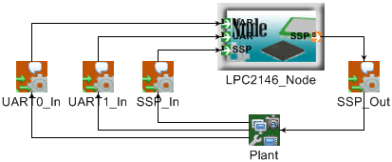
\includegraphics[width=0.80\columnwidth]{figures/QuadrotorHardwarePlatform.png}
\caption{The hardware platform model of AscTec AutoPilot.}
\label{fig:QuadrotorHardwarePlatform}
\end{figure}

The quadrotor helicopter that we use is named AscTec Hummingbird AutoPilot from Ascending Technologies Company \cite{asctech:hummingbird}. The quadrotor's hardware architecture is based on Philips LPC2146. Fig. \ref{fig:QuadrotorHardwarePlatform} illustrates the hardware platform model. The processor LPC2146 is based on an ARM7TDMI-S CPU with two UARTs, SPI, SSP, and other peripherals. The peripherals are modeled in the diagram as objects connecting the input and output ports on the processor to the object representing the plant dynamics. A GPS device is connected through UART1, and a Zigbee module used to receive reference is connected via UART0. The IMU and actuators are connected through SSP. Each device can be configured by setting the \emph{Configuration} attribute of the model object representing the device channel. 

\subsection{Deployment model}

\begin{figure}[!t]
\centering
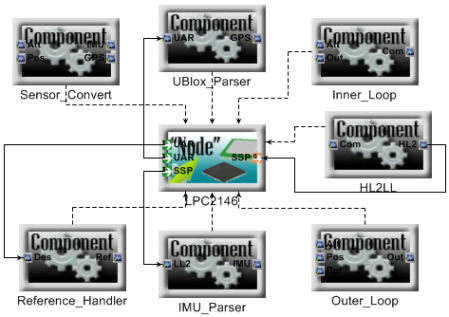
\includegraphics[width=0.80\columnwidth]{figures/QuadrotorDeployment.png}
\caption{The deployment model of control system's software components.}
\label{fig:QuadrotorDeployment}
\end{figure}

In our case study, the model assigns each software component to its own task. In Fig. \ref{fig:QuadrotorDeployment} the dashed connection from a component to a node reference represents an assignment of that component to run as a task on the node. The port connections represent the hardware channel through which that particular message will travel. Local data dependencies are not specified here, as they are represented in the logical software architecture. IChan and OChan objects on the node can also be connected to message objects on a component. These connections represent the flow of data from the physical environment through sensors (IChan objects) or the flow of data back to the environment through actuators (OChan objects).

\subsection{Timing model}

%\begin{figure}[!t]
%\centering
%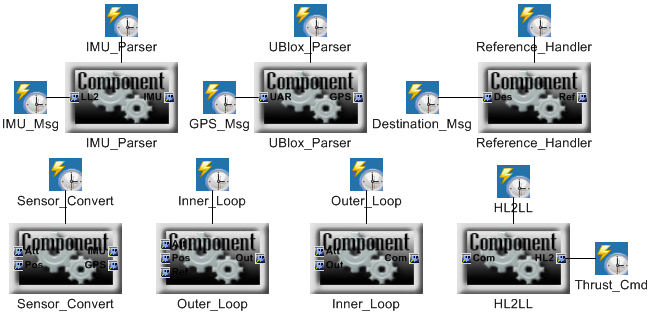
\includegraphics[width=\columnwidth]{figures/QuadrotorTimingModel.png}
%\caption{The timing model of each software component and communication channel.}
%\label{fig:QuadrotorTimingModel}
%\end{figure}

%In Fig. \ref{fig:QuadrotorTimingModel}, 

Each component is assigned a \emph{TTExecInfo} (Time-Triggered Execution Information) object that takes execution period (\emph{ExecPeriod}) and worst case execution time (WCET) (\emph{WCDuration}) as its parameters, and so is each external data transfer. For the processor-local data messages, transfer time is neglected, as reads and writes occur in locally shared memory. The quadrotor is controlled at 1kHz, so the \emph{ExecPeriod} attribute for all components except for \emph{Blox\_Parser} is 1ms. Because the time between two valid data of GPS is longer than 1ms, the \emph{ExecPeriod} for \emph{Blox\_Parser} is 100ms. The worst case latency from sensors to actuators must be smaller than 1ms. Local message transfers may be specified as time-triggered, but in practice they taking place in shared memory are not scheduled. In ESMoL only distributed messages may be scheduled.
 

\subsection{Code generation}

In order to generate the C code based on the TLM in ESMoL, two interpreters are used, which are in Stage 1 and Stage 2 respectively. The Stage 1 interpreter transforms the TLM to an equivalent model in an intermediate language called ESMoL\_Abstract. The model in this intermediate language is flattened and the relationships implied by structures in ESMoL are represented by explicit relation objects in ESMoL\_Abstract \cite{modeling:esmol}.

Stage 2 provides several interpreters, each of which uses the UDM model navigation API to translate the ESMoL\_Abstract model into either code or an analysis model. The deployment model objects are used to generate platform-specific task wrapping and communication code. Shared memory is used to implement the message passing through the ports.

The code generator uses the Google CTemplate engine called from C++ code to perform the generation tasks. We establish a template library containing the initialization codes of different devices. This makes the control system code able to be used on different platforms with a variety of different sensors and actuators. Using the idea of separately generating functional and platform specific code is to realize the platform-based design concept.

Real-Time Workshop (RTW) generates functional ANSI C code for the subsystems specified as Simulink blocks.

Due to the lack of an operating system, we use interrupt-based multi-tasking. The timer interrupt service routine invokes the tasks according to the specified schedule.


\section{Evaluation}

We empirically evaluate the execution time for each component using an external indicator, and timing requirements of these components are met. Each of them takes less than 10$\mu$s during normal operation. We also use $a^3$ tool from the AbsInt Angewandte Informatik company to analyze the WCET and stack usage for each component (seen in Tab. \ref{table:TimingStackAnalyses}). From the table, we can see the total time of analyzed results is 649.7$\mu$s, which is less than 1ms, so the timing requirements can be met.

The memory system consists of 256KB on-chip flash memory (ROM) and 32KB SRAM (RAM). The corresponding binary code is about 110KB, so it fits in the system's ROM space. All the data variables for the communication are preallocated, and from the table we can see the maximum stack usage of a component is 176B. Empirically, we can evaluate that the RAM space is enough for data during normal operation.

\begin{table}
\centering
\caption{Analyzed WCET and stack usage for each component}
\begin{tabular}{|c|c|c|} \hline
Component&WCET ($\mu$s)&Stack Usage (Bytes) \\ \hline
Outer\_Loop & 299 & 176 \\ \hline
Inner\_Loop & 163 & 96 \\ \hline
Sensor\_Convert & 70 & 52 \\ \hline
Reference\_Handler & 0.45 & 4 \\ \hline
UBlox\_Parser & 68.5 & 44 \\ \hline
IMU\_Parser & 19 & 40 \\ \hline
HL2LL & 29.75 & 36 \\ \hline
\end{tabular}
\label{table:TimingStackAnalyses}
\end{table}


\section{Future Work}

Our future work includes: (1) extending the control approach (and software implementation) for group coordination of multiple quadrotor helicopters; (2) modifying ESMoL to support time-triggered wireless network modeling; (3) analyzing the effect of fixed point implementation.




\bibliographystyle{abbrv}
\bibliography{iccps11}

\end{document}
